%%%%%%%%%%%%%%%%%%%%%%%%%%%%%%%%%%%%%%%%%%%%%%%%%%%%%%%%%%%%%%%%%%%%%%%%%%%%%%%%%%%%%%%%%%%%%%%%%%%
\begin{frame}
	\frametitle{Shor}
		\framesubtitle{Overview}

		{\normalsize
		\hspace{0.5cm}{Pick a random number $a < N$.}\\
Compute $gcd(a, N)$. This may be done using the Euclidean algorithm.\\
If $gcd(a, N) \neq 1$, then this number is a nontrivial factor of N, so we are done.
Otherwise, use the period-finding subroutine (below) to find r, the period of the following function:\\
$f(x)=a^{x}{\bmod {N}}$
%i.e. the order {\displaystyle r} r of {\displaystyle a} a in {\displaystyle (\mathbb {Z} _{N})^{\times }} (\mathbb {Z} _{N})^{\times }, %which is the smallest positive integer r for which {\displaystyle f(x+r)=f(x)} f(x+r)=f(x), or {\displaystyle f(x+r)=a^{x+r}{\bmod {N}}%\equiv a^{x}{\bmod {N}}.} {\displaystyle f(x+r)=a^{x+r}{\bmod {N}}\equiv a^{x}{\bmod {N}}.}
%If r is odd, go back to step 1.
%If a r /2 {\displaystyle \equiv } \equiv  −1 (mod N), go back to step 1.
%gcd(ar/2 + 1, N) and gcd(ar/2 - 1, N) are both nontrivial factors of N. We are done.
	}\\
		
		

\end{frame}
%%%%%%%%%%%%%%%%%%%%%%%%%%%%%%%%%%%%%%%%%%%%%%%%%%%%%%%%%%%%%%%%%%%%%%%%%%%%%%%%%%%%%%%%%%%%%%%%%%%

%%%%%%%%%%%%%%%%%%%%%%%%%%%%%%%%%%%%%%%%%%%%%%%%%%%%%%%%%%%%%%%%%%%%%%%%%%%%%%%%%%%%%%%%%%%%%%%%%%%
\begin{frame}
	\frametitle{Shor}
		\framesubtitle{Scheme}
	\vspace{0.5cm}
		\begin{figure}
		\centering
			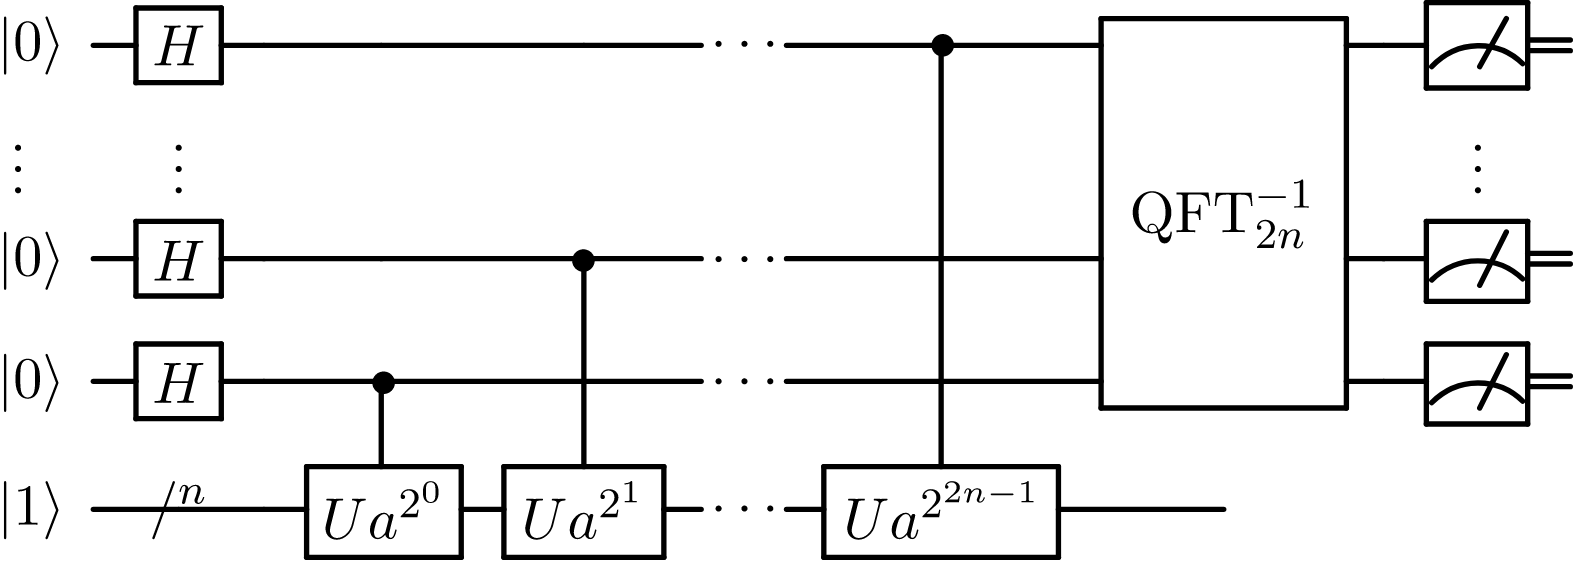
\includegraphics[scale=0.25]{shor}
			\label{fig:shor shor}
		\end{figure}

\end{frame}
%%%%%%%%%%%%%%%%%%%%%%%%%%%%%%%%%%%%%%%%%%%%%%%%%%%%%%%%%%%%%%%%%%%%%%%%%%%%%%%%%%%%%%%%%%%%%%%%%%

%%%%%%%%%%%%%%%%%%%%%%%%%%%%%%%%%%%%%%%%%%%%%%%%%%%%%%%%%%%%%%%%%%%%%%%%%%%%%%%%%%%%%%%%%%%%%%%%%%%
\begin{frame}
	\frametitle{Fast exponentiation}
		\framesubtitle{}

		{\normalsize
		\hspace{0.5cm}{We can calculate $A^{B} mod C$ quickly, using modular multiplication rules:
$$A ^{2} mod C = (A * A) mod C = ((A mod C) * (A mod C)) mod C$$}\\
		}
		

\end{frame}
%%%%%%%%%%%%%%%%%%%%%%%%%%%%%%%%%%%%%%%%%%%%%%%%%%%%%%%%%%%%%%%%%%%%%%%%%%%%%%%%%%%%%%%%%%%%%%%%%%%

%%%%%%%%%%%%%%%%%%%%%%%%%%%%%%%%%%%%%%%%%%%%%%%%%%%%%%%%%%%%%%%%%%%%%%%%%%%%%%%%%%%%%%%%%%%%%%%%%%%
\begin{frame}
	\frametitle{Quantum fourier transform}
		\framesubtitle{}

		{\normalsize
		\hspace{0.5cm}{xyz}\\
		}
		

\end{frame}
%%%%%%%%%%%%%%%%%%%%%%%%%%%%%%%%%%%%%%%%%%%%%%%%%%%%%%%%%%%%%%%%%%%%%%%%%%%%%%%%%%%%%%%%%%%%%%%%%%%